\documentclass{standalone}

\usepackage{tikz}
\usepackage{amsmath}

\begin{document}	
\pagestyle{empty}

\def\layersep{2.5cm}

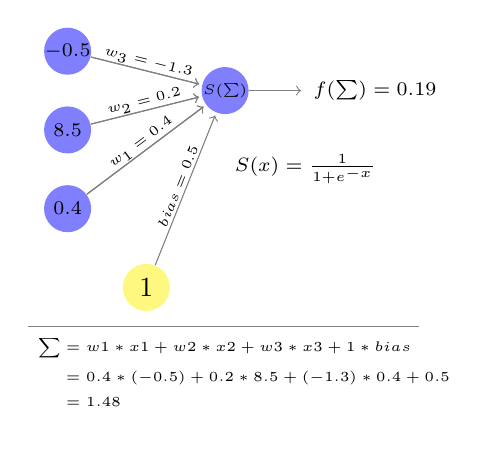
\begin{tikzpicture}[shorten >=1pt,->,draw=black!50, node distance=\layersep]
    \tikzstyle{every pin edge}=[<-,shorten <=1pt]
    \tikzstyle{neuron}=[circle,fill=black!25,minimum size=17pt,inner sep=0pt]
    \tikzstyle{input neuron}=[neuron, fill=green!50];
    \tikzstyle{output neuron}=[neuron, fill=red!50];
    \tikzstyle{hidden neuron}=[neuron, fill=blue!50];
    \tikzstyle{bias neuron}=[neuron, fill=yellow!50];
    \tikzstyle{annot} = [text width=4em, text centered]

	
	\def\inputs{3};
		
	\path[yshift=0.5cm]	node[hidden neuron] (H-1) at (-2,3cm) {}; 
	\node at (H-1) {\scriptsize $-0.5$};
	\path[yshift=0.5cm]	node[hidden neuron] (H-2) at (-2,2cm) {};
	\node at (H-2) {\scriptsize $8.5$};
	\path[yshift=0.5cm]	node[hidden neuron] (H-3) at (-2,1cm) {}; 
	\node at (H-3) {\scriptsize $0.4$};
			
	\node[hidden neuron] (N) at (0, 3){\tiny $S(\sum)$};
	
	
	\path[yshift=0.5cm] node [bias neuron] (B) at (-1, 0 cm) {1}; 
	%\node at (-3.2, 4.5) [anchor=west] {\scriptsize $bias = 0.5$};
	\path (B) edge node [sloped, yshift=3] {\tiny $bias = 0.5$} (N);
	
	% Incoming Links
	\foreach \y in {1,...,\inputs}
		\path (H-\y) edge (N);
		
	
	\path (H-3) edge node [sloped, yshift=3] {\tiny $w_1 = 0.4$} (N);
	\path (H-2) edge node [sloped, yshift=3] {\tiny $w_2 = 0.2$} (N);
	\path (H-1) edge node [sloped, yshift=3] {\tiny $w_3 = -1.3$} (N);
	
	\draw [-] (-2.5, 0) -- (2.5, 0);
	
	\node at (-2.5, -0.6) [anchor=west] {\tiny $\begin{aligned}
				\sum &= w1 * x1 + w2 * x2 + w3 * x3 + 1 * bias  \\
				&= 0.4*(-0.5) + 0.2*8.5 + (-1.3)*0.4 + 0.5\\
		     &= 1.48
		\end{aligned}$};
	
	
	\node at (1, 3) [anchor=west] {\scriptsize $f(\sum) = 0.19$};
	\node at (0, 2) [anchor=west] {\scriptsize $S(x) = \frac{1}{1 + e^{-x}}$};
			
	% Outgoing Link
	\path (N) edge (1, 3);

    
\end{tikzpicture}
% End of code
\end{document}
